\documentclass[14pt]{extreport}
\usepackage{gost}
\usepackage{tikz}
\usepackage{listings}
\usepackage{lscape}
\usetikzlibrary{shapes.geometric}
\begin{document}
\pagenumbering{gobble}% Remove page numbers (and reset to 1)
\begin{landscape}
\vspace*{90px}

\begin{center}
 \Huge{\textbf{МИНИМИЗАЦИЯ ЗАТРАТ ЭНЕРГИИ НА УПРАВЛЕНИЕ УГЛОВЫМ ДВИЖЕНИЕМ СПУТНИКА}}
\end{center}

\vspace*{120px}

\large{Студент 413 группы Исмайылов Гусейн}

\large{Научный руководитель:}

\large{доцент И.А. Панкратов}
\end{landscape}
\newpage
\begin{landscape}
\begin{center}
 \huge{\textbf{ПОСТАНОВКА ЗАДАЧИ ДЛЯ УГЛОВОГО ДВИЖЕНИЯ ТЕЛА}}
\end{center}

\vspace*{40px}

\large{\textbf{Кинематическое уравнение Пуассона}}
\begin{equation}
\LARGE{2\dot{\Lambda}\ =\ \Lambda \circ \Omega}
\end{equation}

\large{\textbf{Граничные условия}}
\begin{equation}
\LARGE{\Lambda(0)\ =\ \Lambda^0}
\end{equation}

\begin{equation}
\LARGE{\Lambda(T)\ =\ \Lambda^T}
\end{equation}

\begin{equation}
\huge{I\ =\ \int_{0}^{T}(\alpha_1\omega_1\ +\ \alpha_2\omega_2\ +\ \alpha_3\omega_3)dt \rightarrow \min}
\end{equation}
\end{landscape}
\newpage
\begin{landscape}
\begin{center}
 \huge{\textbf{АНАЛИТИЧЕСКАЯ ЧАСТЬ РЕШЕНИЯ}}
\end{center}

\begin{center}
\Large{Воспользуемся методом максимума Понтрягина.}
\end{center}

\large
\begin{center}
 $\Huge{\Downarrow}$
\end{center}

\begin{center}
\Large{Получаем краевую задачу}
\end{center}

\begin{equation}
\begin{cases}
\Large{2\dot{\Lambda}\ =\ \Lambda\ \circ\ \Omega,} \\
\Large{2\dot{\Psi}\ =\ \Psi\ \circ\ \Omega,} \\
\Large{\Omega\ =\ \bigg(0\ ,\bigg(\dfrac{p_1}{4\alpha_1},\ \dfrac{p_2}{4\alpha_3},\ \dfrac{p_3}{4\alpha_3}\bigg) \bigg),} \\
\Large{\Lambda(0)\ =\ \Lambda^0,} \\
\Large{\Lambda(T)\ =\ \Lambda^T,}
 \end{cases}
\end{equation}
где 

\begin{equation}
\begin{cases}
\Large{p_1\ =\ - \psi_0\lambda_1\ +\ \psi_1\lambda_0\ +\ \psi_2\lambda_3\ -\ \psi_3\lambda_2,} \\
\Large{p_2\ =\ - \psi_0\lambda_2\ -\ \psi_1\lambda_3\ +\ \psi_2\lambda_0\ +\ \psi_3\lambda_1,} \\
\Large{p_3\ =\ - \psi_0\lambda_3\ +\ \psi_1\lambda_2\ -\ \psi_2\lambda_1\ +\ \psi_3\lambda_0.}
 \end{cases}
\end{equation}
\end{landscape}

\newpage
\large
\begin{landscape}
\begin{center}
 \huge{\textbf{ЧИСЛЕННАЯ ЧАСТЬ РЕШЕНИЯ}}
\end{center}

\begin{center}
\Large{Воспользуемся методом Ньютона.}
\end{center}

\begin{center}
 $\Huge{\Downarrow}$
\end{center}

\begin{center}
\Large{Получаем на i-ой итерации задачу Коши вида}
\end{center}

\begin{equation}
\begin{cases}
2\dot{\Lambda}\ =\ \Lambda\ \circ\ \Omega, \\
2\dot{\Psi}\ =\ \Psi\ \circ\ \Omega,\\
\Lambda(0)\ =\ \Lambda_0^{(i)},\\
\Psi(0)\ =\ \Psi_0^{(i)},\\
\Omega(0)\ =\ \Omega_0^{(i)}.
 \end{cases}
\end{equation}

\begin{center}
Для решения (7) воспользуемся Рунге --- Кутты 4-го порядка.
\end{center}

\end{landscape}

\newpage
\Large
\begin{landscape}
\begin{center}
\Large{Исследование решений при малых углах поворота}
\end{center}
\begin{center}
 \textbf{1) Случаи разных временных отрезков}
\end{center}
\begin{equation}
 \alpha = 10^{\circ}, \ \beta = 8^{\circ},\ \gamma = 5^{\circ}, 
\end{equation}
\begin{equation}
 \widetilde{\alpha} = 0^{\circ}, \ \widetilde{\beta} = 0^{\circ},\ \widetilde{\gamma} = 0^{\circ}, 
\end{equation}
\begin{center}
 Пусть требуется решить задачу с точностью $\varepsilon\ =\ 10^{-9}$
при фиксированных $\alpha_1\ =\ 1000,\ \alpha_2\ =\ 2000,\ \alpha_3\ =\ 3000$. 
\end{center}
\end{landscape}

\newpage
\begin{landscape}
\begin{center}
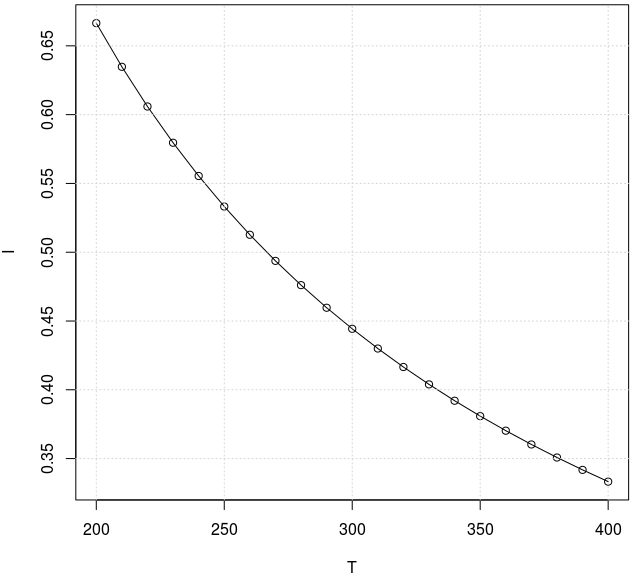
\includegraphics[width=15cm, height=15cm]{lat.png}
\end{center}
\end{landscape}

\newpage
\begin{landscape}
\begin{center}
\textbf{2) Случаи разных весовых множителей функционала качества}
\end{center}
\begin{center}
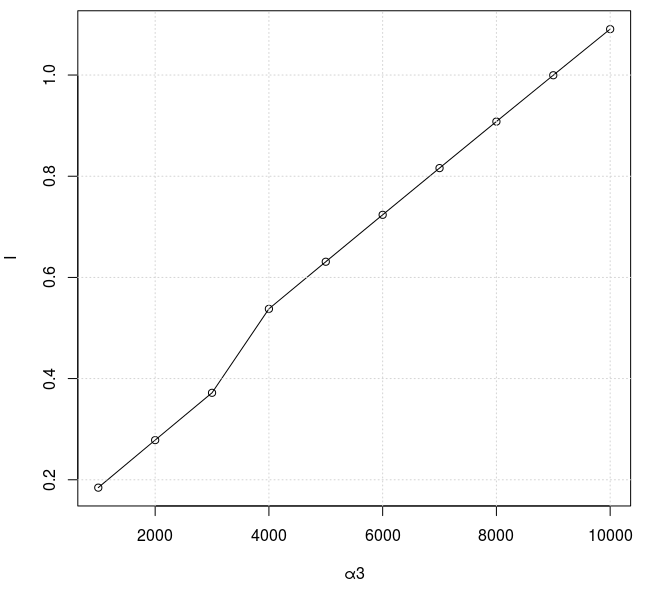
\includegraphics[width=15cm, height=15cm]{laa1.png}
\end{center}
\end{landscape}

\newpage
\begin{landscape}
\begin{center}
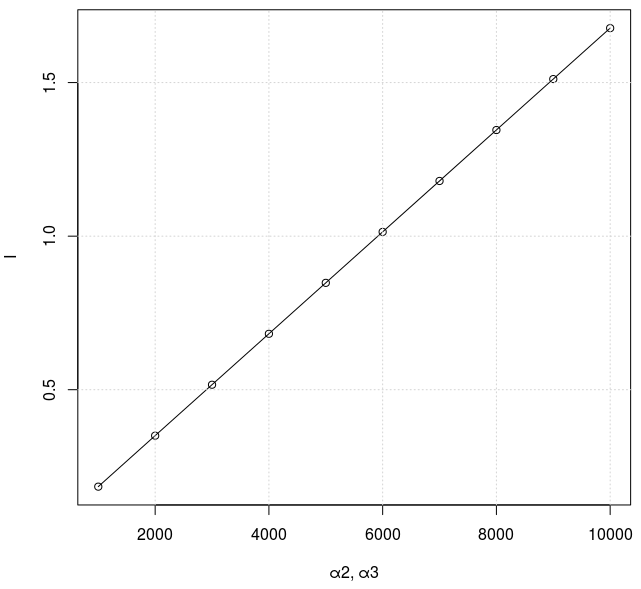
\includegraphics[width=15cm, height=15cm]{laa2.png}
\end{center}
\end{landscape}

\newpage
\begin{landscape}
\begin{center}
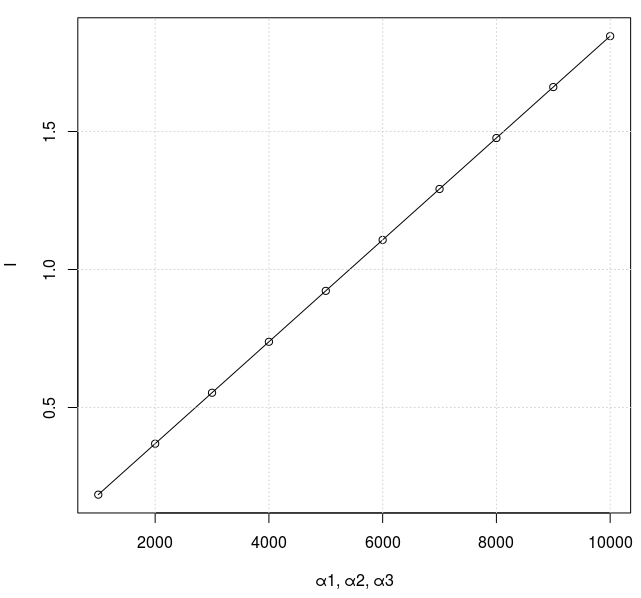
\includegraphics[width=15cm, height=15cm]{laa3.png}
\end{center}
\end{landscape}

\newpage
\begin{landscape}
\begin{center}
\textbf{3) Случаи разных начальных углов поворота}
\end{center}
\begin{center}
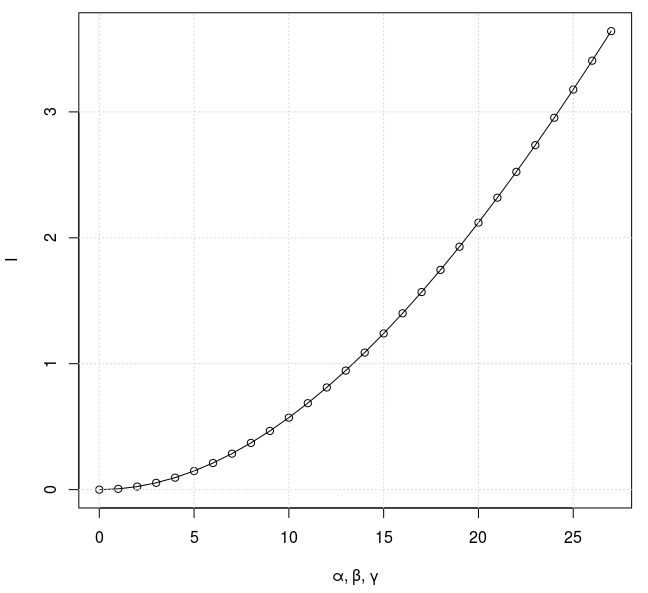
\includegraphics[width=15cm, height=15cm]{va.png}
\end{center}
\end{landscape}

\newpage
\begin{landscape}
\begin{center}
\textbf{Примеры для больших углов поворота}
\end{center}

Пусть требуется решить задачу с точностью $\varepsilon = 10^{-9}$ при весовых множителях $\alpha_1 = 1000,\ \alpha_2 = 2000,\ \alpha_3 = 3000$
для $T\ =\ 300c$, $\alpha\ =\ -78.4^{\circ},\ \beta\ =\ -39.9^{\circ},\ \gamma\ =\ 112.9^{\circ}$.
\begin{equation}
\begin{cases}
2\dot{\Lambda}\ =\ \Lambda \circ \Omega,\\
 \Lambda(0)\ =\ \Lambda^{0}(\lambda_0^{0},\ (\lambda_1^{0},\ \lambda_2^{0},\ \lambda_3^{0})), \\
 \lambda_{0}^{0}\ =\ -0.5821271946729387, \\
 \lambda_{1}^{0}\ =\ 0.10821947847990215, \\
 \lambda_{2}^{0}\ =\ 0.641192910029563, \\
 \lambda_{3}^{0}\ =\-0.48814764756943485. \\
 \Lambda(T)\ =\ \Lambda^{T}(\lambda_0^{T},\ (\lambda_1^{T},\ \lambda_2^{T},\ \lambda_3^{T})), \\
 \lambda_{0}^{T}\ =\ 1, \ 
 \lambda_{1}^{T}\ =\ 0, \ 
 \lambda_{2}^{T}\ =\ 0, \ 
 \lambda_{3}^{T}\ =\ 0. \ 
 \end{cases}
\end{equation}
\end{landscape}

\begin{landscape}
\begin{center}
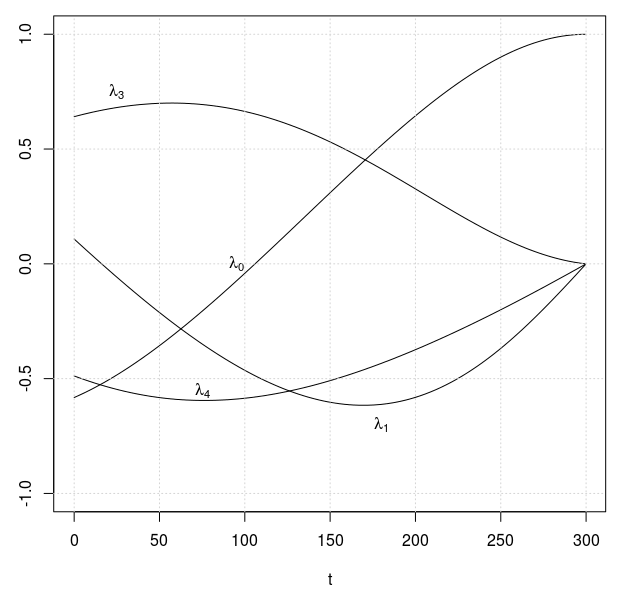
\includegraphics[width=15cm, height=15cm]{l300.png}
\end{center}
\end{landscape}

\begin{landscape}
\begin{center}
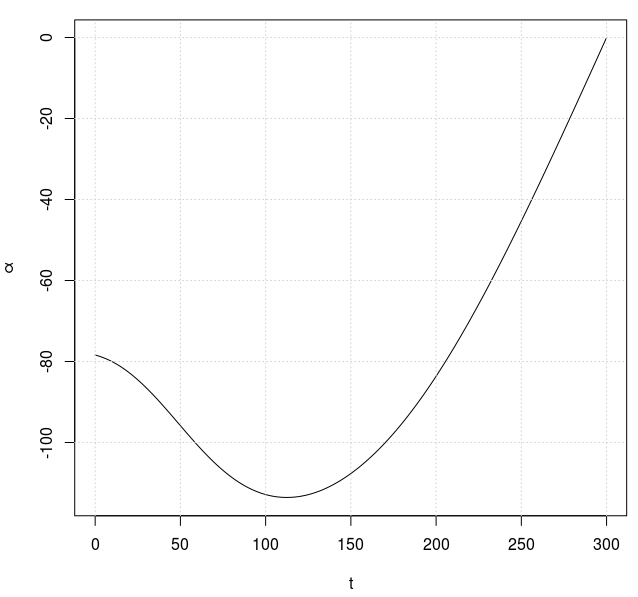
\includegraphics[width=15cm, height=15cm]{alpha.png}
\end{center}
\end{landscape}

\begin{landscape}
\begin{center}
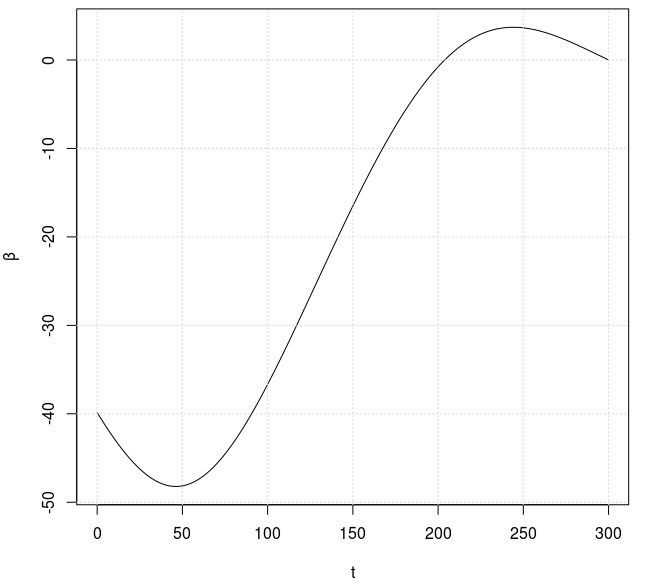
\includegraphics[width=15cm, height=15cm]{beta.png}
\end{center}
\end{landscape}

\begin{landscape}
\begin{center}
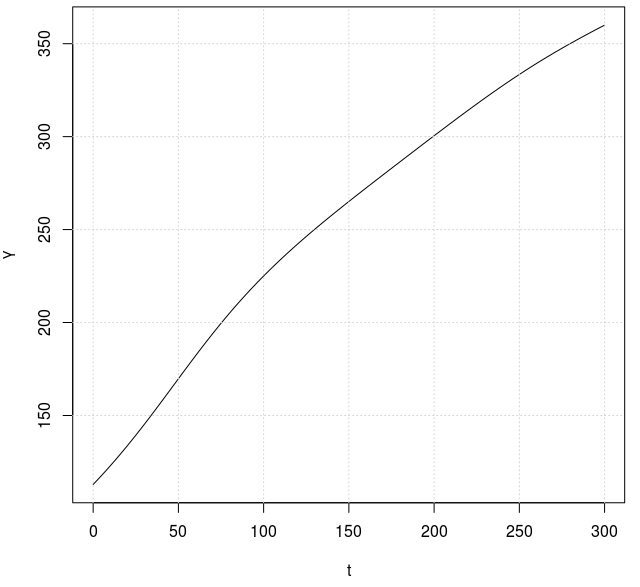
\includegraphics[width=15cm, height=15cm]{gamma.png}
\end{center}
\end{landscape}

\begin{landscape}
\begin{center}
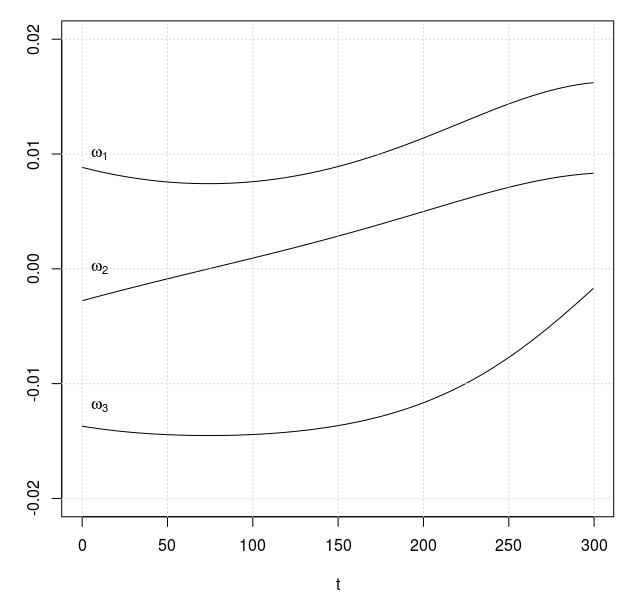
\includegraphics[width=15cm, height=15cm]{o300.png}
\end{center}
\end{landscape}

\newpage
\begin{landscape}
\vspace*{190px}
\begin{center}
 \Huge{\textbf{СПАСИБО ЗА ВНИМАНИЕ}}
\end{center}
\end{landscape}

\end{document}
